\documentclass[a4paper,kul]{kulakarticle} %options: kul or kulak (default)

\usepackage[utf8]{inputenc}
\usepackage[dutch]{babel}

\date{Academiejaar 2021 -- 2022}
\address{
	Industriële Ingenieurswetenschappen \\
	Trillingen \& Golven \\
	Maarten Vanierschot}
\title{Afleidingen}
\author{Robbe Decapmaker}
\usepackage{hyperref}
\usepackage{graphicx}
\usepackage{amsmath, amssymb, amsthm}
\usepackage{siunitx}
\usepackage{flafter} 
\usepackage{pdfpages}
\usepackage{pgfplots}


\begin{document}

\maketitle

\section*{Inleiding}

De afleidingen voor trillingen en golven. 

\section{Afleiding 1}

\textbf{Afleiding van de uitdrukking voor de verplaatsing van een ongedempte trilling aan de hand van de bewegings-vergelijking}\\
\begin{figure}[htbp]
	\centering
	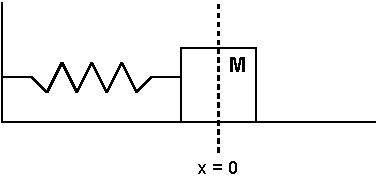
\includegraphics[width=0.4\linewidth]{MassaVeer}
	\caption[Massa veer systeem]{Massa veer systeem}
	\label{fig:massaveer}
\end{figure}
\begin{figure}[htbp]
	\centering
	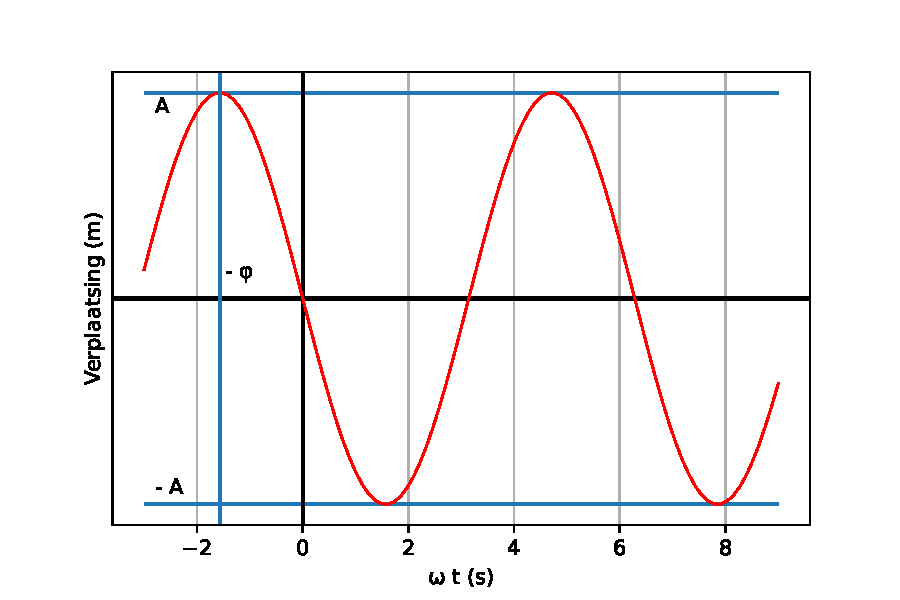
\includegraphics[width=0.7\linewidth]{Harmonische_Oscillator}
	\caption[Harmonische Oscillator]{Harmonische Oscillator}
	\label{fig:harmonischeoscilator}
\end{figure}

We stellen eerst de tweede wet van Newton op voor het blokje M uit figuur \ref{fig:massaveer}.
\begin{equation*}
	\sum \vec{F} = m\vec{a}
\end{equation*}
We kijken nu enkel naar de x-component, en brengen we de kracht van de veer in rekening:
\begin{equation*}
	-kx = m\frac{d^2x}{dt^2}
\end{equation*}
We hebben ook de versnelling geschreven als de tweede afgeleide van de verplaatsing. Door alle termen naar het linker lid te verplaatsen krijgen we volgende differentiaal vergelijking: 
\begin{equation}
	m\frac{d^2x}{dt^2} + kx = 0
	\label{eq:DVGLTrilling}
\end{equation}
Deze differentiaal vergelijking moeten we oplossen aan de hand van beginvoorwaarden. Deze voorwaarden verkrijgen we experimenteel. Bij het experiment noteren we de uitwijking tegenover de tijd. Hierdoor verkrijgen we figuur \ref{fig:harmonischeoscilator}.
Wiskundig vertaalt dit zich tot: 
\begin{equation}
	x(t) = A cos(\omega t + \varphi)
	\label{eq:trilling}
\end{equation}
we kunnen vergelijking \ref{eq:trilling} afleiden om de snelheid van het blokje te verkrijgen: 
\begin{equation}
	v(t) = \frac{dx(t)}{dt} = -\omega Asin(\omega t + \varphi)
	\label{eq:trillingsnelheid}
\end{equation}
Door nogmaals vergelijking \ref{eq:trillingsnelheid} nogmaals af te leiden kunnen we ook de versnelling van het blokje verkrijgen:
\begin{equation}
	a(t) = \frac{d^2x(t)}{dt^2} = -\omega^2 Acos(\omega t + \varphi)
	\label{eq:trillingversnelling}
\end{equation}
Nu kunnen we vergelijkingen \ref{eq:trillingversnelling} en \ref{eq:trilling} invullen in vergelijking \ref{eq:DVGLTrilling}:
\begin{equation}
	-\omega^2 mAcos(\omega t + \varphi) + k A cos(\omega t + \varphi) = 0
	\label{eq:Bewegingsvergelijking}
\end{equation}
Vergelijking \ref{eq:Bewegingsvergelijking} is nu een oplossing voor differentiaal vergelijking \ref{eq:DVGLTrilling} als aan volgende voorwaarde voldaan is:
\begin{align*}
	-\omega^2 mAcos(\omega t + \varphi) + k A cos(\omega t + \varphi) & = 0\\
	(\frac{k}{m}-\omega^2)A cos(\omega t + \varphi) & = 0\\
	\frac{k}{m}-\omega^2 & = 0\\
	\frac{k}{m} & = \omega^2
\end{align*}


\newpage
\section{Afleiding 2}
\textbf{Afleiding van de potentiële en kinetische energie van een ongedempte trilling in functie van de tijd en de plaats}
\\

Er zijn 2 vormen van energie aanwezig in een massa-veer-systeem. We hebben de potentiële energie in de veer en de kinetische energie van het blokje.
\begin{align*}
	E = & \frac{1}{2}kx^2 + \frac{1}{2}mv^2\\
	E(x) = & \frac{1}{2}k A^2cos^2(\omega t +\varphi) + \frac{1}{2}m \omega^2 A^2 sin^2(\omega t + \varphi)\\
	E(x) = & \frac{1}{2}k A^2cos^2(\omega t +\varphi) + \frac{1}{2}m \frac{k}{m} A^2 sin^2(\omega t + \varphi)\\
	E(x) = & \frac{1}{2} k A^2 (cos^2(\omega t +\varphi) + sin^2(\omega t + \varphi))\\
	E(x) = & \frac{1}{2} k A^2
\end{align*} 
We zien nu duidelijk dat de hoeveelheid energie niet afhankelijk is van de uitwijking van de massa. Met andere woorden, de energie blijft constant in het systeem.
\newpage
\section*{Besluit}

Afsluitende tekst.

\end{document}
